% Created 2024-01-13 Sat 15:59
% Intended LaTeX compiler: xelatex
\documentclass[11pt]{article}
\usepackage{graphicx}
\usepackage{longtable}
\usepackage{wrapfig}
\usepackage{rotating}
\usepackage[normalem]{ulem}
\usepackage{amsmath}
\usepackage{amssymb}
\usepackage{capt-of}
\usepackage{hyperref}
\usepackage{xeCJK}
\setCJKmainfont{Heiti SC}
\author{Chen Chen}
\date{\today}
\title{OCCT OCAF}
\hypersetup{
 pdfauthor={Chen Chen},
 pdftitle={OCCT OCAF},
 pdfkeywords={},
 pdfsubject={},
 pdfcreator={Emacs 29.1 (Org mode 9.7)}, 
 pdflang={English}}
\begin{document}

\maketitle
\tableofcontents

\section{OCAF (OpenCascade Application Framework)}
\label{sec:org4d6b0c6}

OCAF 模块提供了一种在 CAD 应用中组织和管理数据的框架。OCAF 的设计目标是提供一个灵活的、可扩展的、支持版本控制的数据模型,以便更容易地创建和管理复杂的 CAD 数据。
\subsection{Purpose of OCAF}
\label{sec:orgfa06bf8}

一般来说,要开发一个设计软件,我们需要提前想清楚如下一些问题:

\begin{itemize}
\item 软件的架构是怎样的?有哪些 components,组件间如何交互
\item 软件的数据模型是怎样的?如何组织软件中的各种数据
\item 如何保持 data model 与 viewer 之间的同步
\item 如何支持 undo/redo 功能
\item 如何持久化软件数据
\end{itemize}

OCAF 模块为上面这些设计问题,提供了解决方案。
\subsection{OCAF 依赖与 OCCT 的其他 modules}
\label{sec:org89c7a89}

\begin{itemize}
\item \texttt{Shape} from \texttt{Modeling Data} module
\item \texttt{Viewer} from \texttt{Visualization} module
\item Modeling functions from \texttt{Modeling Algorithms} module
\end{itemize}
\subsection{OCAF Architecture}
\label{sec:org0852e15}

\begin{center}
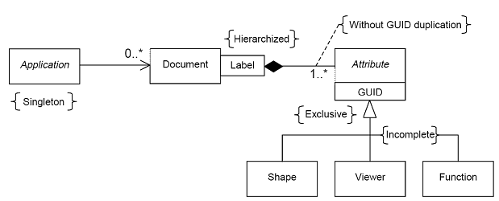
\includegraphics[width=.9\linewidth]{./img/application-document-attribute-model.png}
\end{center}

\begin{itemize}
\item 一个设计软件只有一个 \texttt{Application} 实例
\item \texttt{Application} 实例可以若干个 \texttt{Document}
\item 一个 \texttt{Document} 是一个 \texttt{Label} tree,可以包含多个 Labels
\item 一个 \texttt{Label} 包含了若干个 \texttt{Attribute}
\item 一个 \texttt{Attribute} 实例可以是 \texttt{Shape}, \texttt{Viewer}, \texttt{Function} 中的一种
\end{itemize}
\subsubsection{Application}
\label{sec:org25a552d}

\texttt{Application} 是负责管理文档的抽象类。其主要职责有:

\begin{itemize}
\item 创建文档
\item 保存文档
\item 打开文档
\item 初始化文档视图
\end{itemize}
\subsubsection{Document}
\label{sec:org213a84b}

\texttt{Document} 是承载 App 数据的容器,主要职责有:

\begin{itemize}
\item 管理数据的变更通知
\item Update external link \#不太懂
\item 管理数据的保存与加载
\item store the names of software extensions \#不太懂
\item 管理 command transactions (command 一般指修改操作)
\item 管理 Undo/Redo 选项
\end{itemize}

\texttt{Document} 以一定的 format 保存为 ASCII 文件。通过 reference key,一个文档内可以引用另一个文档中的 label。
\subsubsection{Attribute}
\label{sec:orgab845ca}

All Attributes are organized by the OCAF Data Framework. The Data Framework references all attributes using persistent identifiers in a single hierarchy. (感觉 Data Framework 像一个 Allocator)

软件数据实际上存储在 Attributes 上。Attributes 包含多种继承子 \texttt{Attribute} abstract class 的类型:
\begin{enumerate}
\item Standard attributes
\label{sec:org28f0579}

Standard attributes 涵盖了

\begin{itemize}
\item Simple common data-types: integer, real, string, arrays
\item 辅助功能的 types: tag sources attribute for the children of the label counter.
\item 创建依赖的 types: reference, tree node
\end{itemize}
\item Shape attributes
\label{sec:orgf1df24e}

Shape attributes 包含了建模的几何数据,以及 shape reference, shape evolution tracking 等数据。

还有一些其他的几何数据:
\begin{itemize}
\item \textbf{Datums (基准)} (points, axis, plane)
\item \textbf{Constraints} (tangent-to, at-a-given-distance, from-a-given-angle, concentric, etc.)
\end{itemize}
\item Visualization attributes
\label{sec:org8368571}

Visualization attributes 包含了一些用于 graphical data representation 的数据类型,如 viewer information, visual representation of objects, 以及 auxiliary visual info.
\item Function services
\label{sec:org4b7b39e}

\begin{itemize}
\item The purpose of these attributes is to rebuild objects after they have been modified (parameterization of models).
\item While the \emph{document} manages the notification of changes, a \emph{function} manages propagation of these changes.
\item The function mechanism provides links between functions and calls to various algorithms.
\end{itemize}
\end{enumerate}
\subsection{Reference-key model}
\label{sec:orgf9e511b}

Reference-key driven model V.S. Topology driven model

\begin{center}
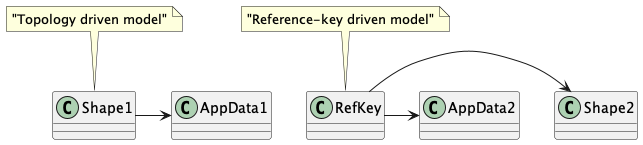
\includegraphics[width=.9\linewidth]{img/reference-key-model.png}
\end{center}

In most existing geometric modeling systems, the data are topology driven. They usually use a BRep, where geometric models are defined by a collection of faces, edges and vertice, to which app-data are attached.

In OCAF, the data are reference-key driven. It is a uniform model in which reference-keys are the persistent identification of data. All data are implemented as attributes attached to ref-keys. 通过一个 ref-key, 多个 attributes 被关联在一起。
\subsubsection{Ref-keys 创建途径: 程序创建和用户创建}
\label{sec:org35e2055}

\begin{itemize}
\item As an application developer, you generate reference-keys in order to give semantics to the data.
\begin{itemize}
\item For example, a function building a prism may create three ref-keys:
\begin{itemize}
\item one for the base of the prism,
\item a second for the lateral faces
\item a third for the top face.
\item these ref-keys makes up a semantic for the prism feature.
\end{itemize}
\end{itemize}
\item The end-user can set a texture to a face he selects, and a ref-key to the face will be created.
\begin{itemize}
\item 当你为所选 face/edge/vertex 创建 ref-key 时,OCAF会自动附加一个 Naming attribute, 用于标注所选 topo.
\end{itemize}
\end{itemize}

在 parametrized modeling 中,当你修改了一个 parameter value,一个 topo element 可能会发生平移。这时通过 ref-key 关联的 data 也会相应更新。
\section{The Data Framework}
\label{sec:orgf02c9f8}

OCAF 中的一些关键 packages 有:

\begin{itemize}
\item \textbf{TDF (Data Framework)}

提供了一种用于存储和管理通用数据的框架,是 OCAF 的核心包,定义了文档、标签、数据存储等概念。
提供了基本的数据存储和版本控制机制。

它定义了数据模型的基本概念,如标签、数据类型等。

\item \textbf{TDocStd (Technology Document Standard)}

\texttt{TDocStd} 提供了文档和存储的概念。它定义了如何组织和管理存储在文档中的数据。

\item \textbf{XCAF (Extended Computer-Aided Facilities)}

\texttt{XCAF} 提供了对扩展数据的支持,包括属性、引用和组件的概念。它使用户能够为几何模型添加附加信息。

\item \textbf{TFunction}

\texttt{TFunction} 允许用户将功能与数据关联,使得模型的操作和行为更加动态和可定制。

\item \textbf{TPrsStd (Technology Presentation Standard)}

\texttt{TPrsStd} 提供了用于在用户界面中显示和呈现几何模型的工具。
\end{itemize}
\subsection{学习步骤}
\label{sec:org1e7e4f6}

\begin{itemize}
\item 先了解 \texttt{TDF} 的基本概念,包括标签、数据类型和版本控制。为后续学习奠定基础。
\item 学习使用 \texttt{TDocStd} 创建、管理和保存文档。了解如何在文档中存储数据,并理解版本控制的原理。
\item 学习使用 \texttt{XCAF} 扩展数据,包括属性、引用和组件。让你能够为几何模型添加附加信息,使其更丰富和灵活。
\item 学习使用 \texttt{TFunction} 将功能和操作关联到模型。让你更灵活地处理和操作几何模型。
\item 学习使用 \texttt{TPrsStd} 在用户界面中呈现和显示几何模型,包括创建图形视图以及将模型呈现到用户界面中。
\end{itemize}
\subsection{TDF package}
\label{sec:org2d7df14}


\subsection{TDocStd package}
\label{sec:org8847fa4}

\subsection{XCAF package}
\label{sec:org88bed77}

\subsection{TFunction package}
\label{sec:orgb10568f}

\subsection{TPrsStd package}
\label{sec:org32642c9}
\end{document}
